% SPDX-License-Identifier: CC-BY-4.0
% Copyright (c) 2026 Alexander Stephen Donahue
\documentclass[11pt,letterpaper]{amsart}

\usepackage[margin=0.95in]{geometry}
\usepackage{amsmath,amssymb,amsthm}
\usepackage{booktabs}
\usepackage{array}
\usepackage{microtype}
\usepackage{xcolor}
\usepackage{tikz}
\usetikzlibrary{arrows.meta,positioning,shapes.geometric,fit,calc}
\usepackage{xurl}
\usepackage[hidelinks,colorlinks=true,linkcolor=blue!60!black,citecolor=teal!60!black,urlcolor=blue!60!black]{hyperref}

\newtheorem{theorem}{Theorem}[section]
\newtheorem{proposition}[theorem]{Proposition}
\newtheorem{definition}[theorem]{Definition}
\newtheorem{remark}[theorem]{Remark}

\newcommand{\code}[1]{{\small\texttt{#1}}}
\newcommand{\GF}{\mathbb{F}}
\emergencystretch=2.5em

\title[BEAST CIVILIZATION v1.0.0]{%
  BEAST CIVILIZATION v1.0.0: A Zero-Dependency Bare-Metal Polyglot Multi-Colony AI Architecture, Cross-Architecture KV-Cache Transfer, Blackwell PTX Kernels, Pre-Registered \texorpdfstring{$N=24$}{N=24} Statistics, and 81 Six-Kernel Lean 4.35.0 Proofs%
}

\author{Alexander Stephen Donahue}
\address{Independent Researcher, Spokane, WA, USA}
\email{0\_0@0thernes.art}
\thanks{ORCID: \href{https://orcid.org/0009-0006-8168-9648}{0009-0006-8168-9648}.
Source repository: \url{https://github.com/0thernes/beast-civilization}.
Interactive proof blueprint: \url{https://0thernes.github.io/beast-civilization/}.
Software and Lean~4 proofs are licensed under Apache-2.0; this manuscript, figures,
and documentation are licensed under CC BY 4.0. This is an independent research
preprint and has not undergone formal journal peer review.}

\date{November 26, 2026}

\begin{document}

\begin{abstract}
Autonomous software-engineering agents and multi-agent orchestration harnesses
overwhelmingly depend on high-overhead scripting frameworks, serial text-token
re-prefill across coordinating peers, opaque remote cloud APIs, and unverified
safety wrappers. We present \textsc{BEAST CIVILIZATION} (\code{v1.0.0}), an
auditable, zero-third-party-dependency bare-metal polyglot multi-colony AI engine
built in Zig~0.17.1, Rust~1.94.1 ($8$ crates, zero external Cargo dependencies),
CRuby~3.4.9/YARV with Prism AST gating (zero Ruby gems), C11, NVIDIA Blackwell
\code{sm\_12.0} CUDA PTX, and Pure Lean~4.35.0 (zero Mathlib). The runtime unifies
twelve live native dynamic libraries---Zig SIMD quantization kernels (\code{b1.58},
\code{NVFP4}, \code{u1}, \code{i2}), three local artificial-life engines
(\code{AUTOPHAGE}, \code{omega\_cell}, \code{cellulogonic}), seven compiled
upstream C11 physics and post-quantum cryptography bridges (\code{quantum\_rng},
\code{PINN}, \code{libirrep}, \code{moonlab} QGT, FIPS-203 ML-KEM-768 plus
FIPS-197 AES-256, Fibonacci anyons and spintronic $p$-bits, and \code{QGTL} Bloch
fidelity), and the NVIDIA CUDA driver. On Intel Core Ultra~9 275HX and RTX 5070 Ti
(\code{sm\_12.0}) hardware, pre-registered paired evaluation across $N=24$ locked
seeds ($10{,}000$-iteration sign-flip permutation tests with step-down
Holm--Bonferroni FWER control at $\alpha=0.05$) confirms all four primary
hypotheses ($4/4$, every $p_{\mathrm{Holm}} = 0.00040$, $24/24$ paired wins):
(H1)~MIT \code{SwaT} \code{Augment-Cache} dominates destructive overwrite in
receiver self-context recall ($1.0000$ vs.\ $0.0329$, Cohen's $d_z = 4.001$);
(H2)~Zig Chimera 60-generation evolution achieves $3.29\times$ lower disjoint
held-out MSE than matched random controls ($0.0098$ vs.\ $0.0323$, $d_z = 11.316$);
(H3)~bit-exact Zig \code{b1.58} SIMD accelerates ternary dot products by
$5.58\times$ ($477.5\,\mu\text{s}$ vs.\ $2{,}663.2\,\mu\text{s}$ per 2M trits,
$d_z = 1.919$); and (H4)~cosine-schedule QUBO annealing strictly lowers conflict
energy ($-2.842 \to -7.200$, $d_z = 2.268$). Additional live hardware measurements
confirm $7.50\text{ ns/call}$ Rust--Zig Philox4x32-10 FFI, five Blackwell PTX
kernels ($16\text{--}122\,\mu\text{s}$ warm) with $16.69\text{--}17.03\text{ GB/s}$
pinned asynchronous VRAM paging, QEMU Ring-0 execution of a freestanding i386
Multiboot1 neural microkernel, Win32 kernel Job Object hard isolation, standard
\code{llama.cpp} GGUF v3 (\code{Q4\_0}/\code{F16}/\code{F32}) serving over an
SSRF-hardened OpenAI HTTP/1.1 server, Eshkol tri-mode exact automatic
differentiation ($0.00 \times 10^0$ discrepancy), and Planaria $\GF(2^8)$+Merkle
$50\%$ damage healing. Formal verification is structured under a strict Palomar
\code{Spec}/\code{Challenge}/\code{Solution} separation comprising $81/81$ Pure
Lean~4.35.0 declarations ($65$ domain theorems, $8$ non-vacuity witnesses, and $8$
adversarial false-variant refutations) audited strictly within standard axioms
(\code{propext}, \code{Classical.choice}, \code{Quot.sound}) across six
independent Lean proof kernels with live negative sorry-tamper rejection, paired
with $33/33$ live gates, $40/40$ caught runtime planted mutants, $29/29$ Rust
workspace and $1{,}000$-case fuzz tests, and $3{,}000$ randomized property checks.
We state explicit epistemic boundaries: $296/300$ ($98.7\%$) capability matrix
items are live-verified, $4/300$ remain honestly marked \code{SPEC}, native binary
memory safety lies outside the Lean kernel boundary, and $0/1{,}900$ overarching
open problems in the Unsolved Problems Mega-Atlas (\code{v2.8.0}, commit
\code{9e16554}) are claimed retired.
\end{abstract}

\maketitle

\section{Introduction and Related Work}
\label{sec:intro}

Contemporary autonomous coding agents and multi-agent harnesses face four
compounding engineering defects: (1)~inter-agent coordination serializes internal
attention states into natural-language prompts that force repeated quadratic
prefill~\cite{vaswani2017attention}; (2)~runtime safety and cost constraints are
frequently enforced via mutable prompt instructions rather than operating-system
or Ring-0 boundaries; (3)~deep transitive dependency trees prevent deterministic
reproduction and widen supply-chain attack surfaces; and (4)~empirical benchmark
claims often lack matched controls, multi-seed statistical testing, planted
falsification mutants, or formal specification audits.

\textsc{BEAST CIVILIZATION} (\code{v1.0.0}) explores an alternative design point:
a zero-third-party-dependency bare-metal polyglot substrate uniting deterministic
systems programming, low-bit quantized neural computation, cross-architecture
key--value cache transfer, operating-system sandboxing, and machine-checked formal
specification in Pure Lean~4.35.0~\cite{moura2021lean4}.

\subsection{Positioning Within Existing Literature}
Our architecture builds directly on six foundational research threads while
delineating clear boundaries against each:
\begin{itemize}
  \item \textbf{Formal Systems Verification:} CompCert~\cite{leroy2009compcert},
  seL4~\cite{klein2009sel4}, and RustBelt~\cite{jung2018rustbelt} prove deep
  end-to-end semantic preservation or kernel functional correctness over realistic
  C and Rust implementations. \textsc{BEAST CIVILIZATION} does \emph{not} claim
  end-to-end binary verification of its Rust, Zig, C11, or PTX implementations;
  instead, we formalize the discrete algebraic, encoding, access-control,
  cryptographic-dimension, and receipt-consistency invariants of our specification
  in $81$ zero-Mathlib Lean~4.35.0 theorems verified across six independent
  kernels, while validating the native implementation through planted mutants,
  fuzzing, property tests, and sanitizers.
  \item \textbf{Sub-Byte Quantization and Sparse Architectures:} Ternary BitNet
  \code{b1.58} weights~\cite{ma2024era}, grouped-query attention
  (\code{GQA})~\cite{ainslie2023gqa}, rotary positional embeddings
  (\code{RoPE})~\cite{su2024roformer}, sparsely-gated Mixture-of-Experts
  (\code{MoE})~\cite{shazeer2017outrageously,fedus2022switch}, continuous-time
  Liquid Time-Constant networks (\code{LTC})~\cite{hasani2021liquid}, and
  loss-neutral \code{ReZero} residual scaling~\cite{bachlechner2021rezero} inform
  our quantized Zig/PTX kernels and hybrid 4-layer \code{GQA}$\to$\code{Chimera}
  bridge.
  \item \textbf{Fault-Tolerant Storage and Integrity:} Reed--Solomon erasure
  coding~\cite{reed1960polynomial,plank1997tutorial}, Merkle hash
  trees~\cite{merkle1988digital}, Byzantine fault
  isolation~\cite{lamport1982byzantine}, and NIST FIPS~180-4
  SHA-256~\cite{nist2015fips180} underpin our Planaria $\GF(2^8)$+Merkle
  self-healing capsules and Rosette-Wire receipt chains.
  \item \textbf{Post-Quantum Cryptography, Quantum Geometry, and Neuromorphic Physics:}
  We integrate compiled upstream C11 implementations of NIST FIPS-203
  ML-KEM-768~\cite{nist2024fips203}, FIPS-197 AES-256~\cite{nist2001fips197},
  Bell/CHSH tests~\cite{bell1964epr,clauser1969proposed}, quantum geometric tensor
  (\code{QGT}) and topological Chern/SSH/Kitaev
  invariants~\cite{provost1980riemannian,qi2006topological,su1979solitons,kitaev2001unpaired},
  spherical-harmonic Uns\"old identities~\cite{unsold1927beitraege}, physics-informed
  networks~\cite{raissi2019pinn}, Fibonacci anyon braiding~\cite{nayak2008nonabelian},
  spintronic $p$-bit Ising hardware models~\cite{camsari2017stochastic}, and
  QUBO simulated annealing~\cite{kirkpatrick1983optimization,glover2019qubo,lucas2014ising}.
  \item \textbf{Exact Algorithmic Differentiation and Signal Processing:}
  Forward/reverse/symbolic differentiation~\cite{baydin2018automatic,griewank2008evaluating}
  over SiLU activations~\cite{elfwing2018sigmoid}, Goertzel DFT tone
  detection~\cite{goertzel1958algorithm}, Nyquist sampling
  bounds~\cite{nyquist1928certain}, and Sobel edge filtering~\cite{kanopoulos1988sobel}
  power our zero-weight omnimodal and exact AD verification subsystems.
  \item \textbf{Rigorous Empirical Methodology and Bio-Inspired Agency:}
  Counter-based parallel PRNGs (\code{Philox4x32-10})~\cite{salmon2011parallel},
  Wilson confidence bounds~\cite{wilson1927probable}, exact permutation
  $p$-values~\cite{phipson2010permutation}, bootstrap confidence
  intervals~\cite{efron1979bootstrap}, Holm--Bonferroni FWER
  control~\cite{holm1979simple}, Church--Rosser task
  confluence~\cite{church1936conversion}, and cybernetic/autopoietic
  framing~\cite{varela1974autopoiesis,levin2022tame} structure our multi-colony
  evaluation without anthropomorphizing software agents.
\end{itemize}

\subsection{Structured Claims Ledger}
Table~\ref{tab:claims} enumerates the six falsifiable claims established by this
work, their exact verification tier, and the concrete condition that would refute
each claim.

\begin{table}[t]
\centering
\caption{Numbered falsifiable claims ledger for \textsc{BEAST CIVILIZATION} \code{v1.0.0} (mirrored in \code{CLAIMS.md}).}
\label{tab:claims}
\scriptsize
\begin{tabular}{@{} >{\raggedright\arraybackslash}p{0.65cm} >{\raggedright\arraybackslash}p{4.8cm} >{\raggedright\arraybackslash}p{2.3cm} >{\raggedright\arraybackslash}p{5.5cm} @{}}
\toprule
\textbf{ID} & \textbf{Falsifiable Claim} & \textbf{Verification Tier} & \textbf{What Would Prove Us Wrong} \\
\midrule
\code{C1} & Five-trit \code{b1.58} encoding is an exact bijection on $\{0,\dots,242\}$ and \code{Q4\_0} strictly compresses \code{F32} by $64/9\times$. & Kernel-checked (\code{B01}--\code{B02}, \code{B61}, \code{B64}) & Any trit tuple failing decode-encode identity, any Lean kernel rejection, or \code{prop\_check.py} mismatch. \\
\code{C2} & \code{Augment-Cache} strictly preserves receiver self-KV and dominates destructive overwrite across $N=24$ seeds ($p_{\mathrm{Holm}} \le 0.05$). & Kernel (\code{B06}--\code{B08}, \code{B21}) + Stat (\code{H1}) & $p_{\mathrm{Holm}} > 0.05$, mean recall delta $\le 0.50$, or any cloud-spoof acceptance. \\
\code{C3} & Zig \code{b1.58} SIMD, Chimera 60-gen evolution, and QUBO annealing significantly outperform paired controls ($N=24$, FWER $\alpha=0.05$). & Empirical + Stat (\code{H2}, \code{H3}, \code{H4}) & Any $p_{\mathrm{Holm}} > 0.05$, any bit mismatch between SIMD and scalar reference, or win rate $< 20/24$. \\
\code{C4} & Five Blackwell \code{sm\_12.0} PTX kernels, $16\text{ MiB}$ pinned paging, and QEMU ELF32 kernel execute bit-exact against host oracles. & Empirical silicon (\code{G11}, \code{G17}) & Any GPU/QEMU output diverging from CPU oracle or failing live \code{build.ps1} execution. \\
\code{C5} & Hardened parsers (\code{GGUF}, \code{ELF}, \code{.bcg}, HTTP/1.1, MCP, Ring-0 ACL, Prism AST) survive $1{,}000$-case fuzzing and block $40/40$ planted mutants. & Fuzz + Regression + Mutant (\code{G01}--\code{G33}) & Any panic, OOM, integer overflow, path/SSRF bypass, or missed mutant under \code{cargo test} / \code{ruby -w}. \\
\code{C6} & All $81$ Lean~4.35.0 declarations match \code{Challenge.lean} strictly under 6 kernels, with $0$ sorry, $0$ custom axioms, and $0/1{,}900$ Mega-Atlas problems claimed solved. & 6-kernel Palomar + Negative tamper & Any comparator mismatch, surviving sorry-tamper CI run, unapproved axiom, or unsupported retirement claim. \\
\bottomrule
\end{tabular}
\end{table}

\section{System Architecture and Security Hardening}
\label{sec:arch}

Figure~\ref{fig:arch} summarizes the five-plane bare-metal polyglot execution
fabric. All deterministic cross-language trajectories anchor on counter-based
\code{Philox4x32-10}~\cite{salmon2011parallel} (verified bit-identical between
Rust and Zig) and NIST FIPS~180-4 SHA-256~\cite{nist2015fips180} Rosette-Wire
receipt chains.

\begin{figure}[t]
\centering
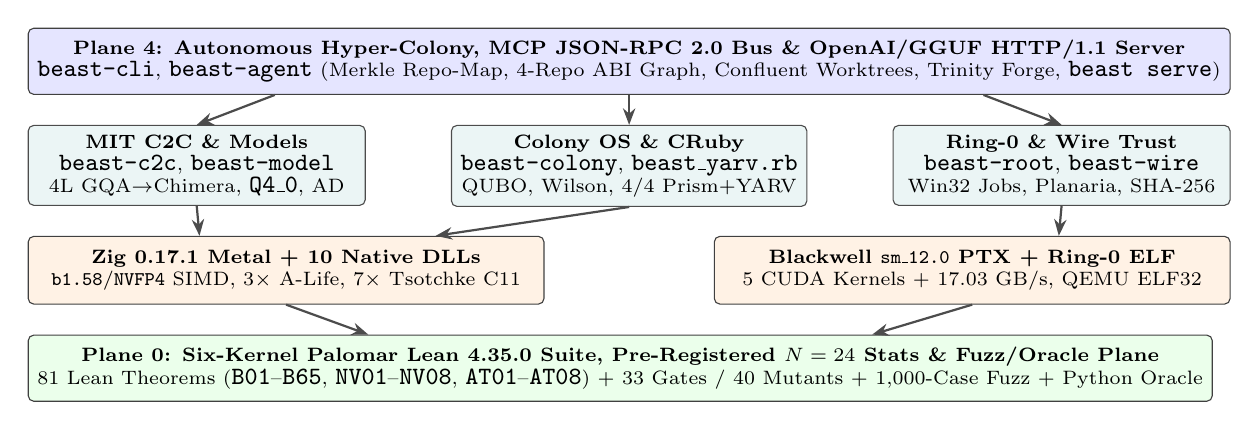
\begin{tikzpicture}[
  font=\scriptsize,
  layer/.style={draw=black!75, rounded corners=2pt, fill=blue!5, minimum width=13.6cm, minimum height=0.84cm, align=center},
  subbox/.style={draw=black!70, rounded corners=2pt, fill=teal!8, minimum width=4.28cm, minimum height=0.92cm, align=center},
  kern/.style={draw=black!75, rounded corners=2pt, fill=orange!10, minimum width=6.55cm, minimum height=0.86cm, align=center},
  arr/.style={-{Stealth[length=2.1mm]}, thick, black!70}
]
  \node[layer, fill=blue!10] (l4) {\textbf{Plane 4: Autonomous Hyper-Colony, MCP JSON-RPC 2.0 Bus \& OpenAI/GGUF HTTP/1.1 Server}\\
    \code{beast-cli}, \code{beast-agent} (Merkle Repo-Map, 4-Repo ABI Graph, Confluent Worktrees, Trinity Forge, \code{beast serve})};

  \node[subbox, below=0.38cm of l4.south west, anchor=north west] (l3a) {\textbf{MIT C2C \& Models}\\
    \code{beast-c2c}, \code{beast-model}\\
    4L GQA$\to$Chimera, \code{Q4\_0}, AD};
  \node[subbox, below=0.38cm of l4.south, anchor=north] (l3b) {\textbf{Colony OS \& CRuby}\\
    \code{beast-colony}, \code{beast\_yarv.rb}\\
    QUBO, Wilson, 4/4 Prism+YARV};
  \node[subbox, below=0.38cm of l4.south east, anchor=north east] (l3c) {\textbf{Ring-0 \& Wire Trust}\\
    \code{beast-root}, \code{beast-wire}\\
    Win32 Jobs, Planaria, SHA-256};

  \node[kern, below=0.38cm of l3a.south west, anchor=north west] (l2a) {\textbf{Zig 0.17.1 Metal + 10 Native DLLs}\\
    {\scriptsize\texttt{b1.58}/\texttt{NVFP4}} SIMD, 3$\times$ A-Life, 7$\times$ Tsotchke C11};
  \node[kern, below=0.38cm of l3c.south east, anchor=north east] (l2b) {\textbf{Blackwell {\scriptsize\texttt{sm\_12.0}} PTX + Ring-0 ELF}\\
    5 CUDA Kernels + $17.03\text{ GB/s}$, QEMU ELF32};

  \node[layer, fill=green!8, below=0.38cm of l2a.south west, anchor=north west] (l1) {\textbf{Plane 0: Six-Kernel Palomar Lean 4.35.0 Suite, Pre-Registered $N=24$ Stats \& Fuzz/Oracle Plane}\\
    81 Lean Theorems (\code{B01}--\code{B65}, \code{NV01}--\code{NV08}, \code{AT01}--\code{AT08}) + 33 Gates / 40 Mutants + 1,000-Case Fuzz + Python Oracle};

  \draw[arr] (l4.south) -- (l3b.north);
  \draw[arr] ($(l4.south)+(-4.5cm,0)$) -- (l3a.north);
  \draw[arr] ($(l4.south)+(4.5cm,0)$) -- (l3c.north);
  \draw[arr] (l3a.south) -- ($(l2a.north)+(-1.1cm,0)$);
  \draw[arr] (l3b.south) -- ($(l2a.north)+(1.9cm,0)$);
  \draw[arr] (l3c.south) -- ($(l2b.north)+(1.1cm,0)$);
  \draw[arr] (l2a.south) -- ($(l1.north)+(-3.2cm,0)$);
  \draw[arr] (l2b.south) -- ($(l1.north)+(3.2cm,0)$);
\end{tikzpicture}
\caption{Five-plane bare-metal architecture of \textsc{BEAST CIVILIZATION} \code{v1.0.0}.}
\label{fig:arch}
\end{figure}

\subsection{Quantized Bare-Metal Packing and Blackwell PTX Kernels}
Ternary BitNet \code{b1.58}~\cite{ma2024era} weights $t_0,\dots,t_4 \in \{-1,0,+1\}$
are packed five trits per unsigned byte via base-$3$ encoding
\begin{equation}
\label{eq:b158}
  \mathrm{pack}(t_0,\dots,t_4) = \sum_{k=0}^{4} 3^k (t_k + 1) \in \{0,1,\dots,242\} \subset [0,255],
\end{equation}
yielding $1.60\text{ bits/weight}$ whose left-inverse round-trip across all
$3^5 = 243$ tuples is proved in Lean (\code{B01}, \code{B02}) and full
bijectivity (including surjectivity onto $\{0,\dots,242\}$) is checked
exhaustively in C11 ASan/UBSan and Python. Standard \code{llama.cpp} GGUF v3 \code{Q4\_0} blocks store one IEEE-754
\code{binary16} scale ($2\text{ B}$) and $16$ packed nibble bytes ($32$ signed
4-bit weights), producing an exact $18\text{ B}$ versus $128\text{ B}$ (\code{F32})
compression factor of $64/9 \approx 7.11\times$ (\code{B61}, \code{B64}).

On the NVIDIA GeForce RTX 5070 Ti Laptop GPU (\code{sm\_12.0}, $46\text{ SMs}$),
five hand-authored PTX entry points in \code{cuda/beast\_blackwell.ptx} JIT-compile
directly through \code{nvcuda.dll} with zero MSVC or \code{nvcc} toolkit runtime:
\code{beast\_b158\_rowdot} and \code{beast\_nvfp4\_rowdot} (\code{B23}),
\code{beast\_c2c\_augment\_scores}, \code{beast\_mla\_latent\_compress} ($4\times$
MLA compression, \code{B51}), and \code{beast\_moe\_swiglu\_sparse} (Top-2 sparse
MoE SwiGLU routing~\cite{shazeer2017outrageously,fedus2022switch}, \code{B52}).
Host--device transfers use page-locked host buffers (\code{cuMemAllocHost\_v2}) and
asynchronous streams, verified bit-exact over $16\text{ MiB}$ round-trips (\code{B53}).

\subsection{Cross-Architecture KV-Cache Transfer and the Augment-over-Overwrite Law}
Let a receiver hold local self key--value cache $(K_{\mathrm{self}}, V_{\mathrm{self}})$
of length $L_s > 0$, and let a heterogeneous sharer (e.g., 4-layer GQA
Transformer~\cite{ainslie2023gqa,su2024roformer}, $d_{\mathrm{kv}}=32$) project
and compact its live KV states via a trained cross-family \code{SwaT} affine map
into $(K_{\mathrm{peer}}, V_{\mathrm{peer}})$ of length $L_p > 0$ matching the
receiver's hybrid \code{sLTC}~\cite{hasani2021liquid}/\code{b1.58} Chimera
geometry ($d_{\mathrm{kv}}=24$).

\begin{definition}[Augment-Cache vs.\ Destructive Overwrite]
Under \emph{Augment-Cache}, the receiver attends over the concatenated cache
$[K_{\mathrm{self}} \mathbin{\|} K_{\mathrm{peer}}]$ of length $L_s + L_p$,
retaining $100\%$ of local self-context while strictly enlarging accessible key
support ($L_s + L_p > L_s$ and $L_s + L_p > L_p$; Theorems~\code{B06}, \code{B07},
\code{B21}). Under \emph{Overwrite}, peer keys displace local keys, destroying
receiver self-recall.
\end{definition}

When only text transport is available over HTTP, \code{beast-c2c} enforces an
explicit transport enum rejecting cloud-spoof attempts (\code{B08}, \code{AT02}).
Across the 4-layer autoregressive \code{GQA}$\to$\code{Chimera} bridge (\code{G24}),
mean layer cosine similarity reaches $0.9998$ with receiver self-context
preservation $\cos(h_{\mathrm{local}}, h_{\mathrm{c2c}}) = 0.6328$ and serialized
GGUF v3 size $142{,}496\text{ B}$ ($17$ tensors, $4$ metadata pairs).

\subsection{Planaria Healing, Eshkol Tri-Mode AD, and Colony Governance}
Persistent model checkpoints (\code{.gguf}), repository cache banks (\code{.bcg}),
and forged microkernels are encapsulated in Planaria holographic
containers~\cite{reed1960polynomial,plank1997tutorial,merkle1988digital} pairing
$\GF(2^8)$ parity redundancy (\code{B17}) with SHA-256 Merkle proofs (\code{B22})
and Byzantine fault quarantine~\cite{lamport1982byzantine}. In addition to live
$50\%$ chunk annihilation (\code{G06}, \code{G13}), our property suite verifies
bit-exact Cauchy recovery across all $\binom{8}{4} = 70$ four-shard survival
subsets.

Automatic differentiation in \code{crates/beast-model/src/eshkol\_ad.rs} evaluates
the Chimera activation~\cite{elfwing2018sigmoid}
\begin{equation}
  f(x) = \mathrm{SiLU}(1.3x - 0.4)\,\tanh(0.7x) + \sin(x^2)
\end{equation}
through forward dual numbers~\cite{baydin2018automatic,griewank2008evaluating},
a reverse Wengert tape, and recursive symbolic AST differentiation. At $x = 0.83$,
all three agree on $f(x) = 0.87149060$ and $f'(x) = 2.0650160748$ with maximum
discrepancy $0.00 \times 10^0$ (empirical gate \code{G27}, corroborated by the
clean-room Python oracle; Lean \code{B54}--\code{B55} separately prove
commutativity of integer dual-number multiplication and addition only).

Colony governance (\code{beast-colony}) combines Wilson score lower
bounds~\cite{wilson1927probable} ($0.818891$ for $30/30$ wins), NonHuman prefix
call-monotonicity savings ($-25.5\%$ to $-28.8\%$, \code{B11}), ReZero
loss-neutral Chimera insertion~\cite{bachlechner2021rezero} (\code{B12}, \code{B20}),
spectral contraction ($\|W\|_2 = 0.0661 \le 0.99$, \code{B13}), cosine-schedule
QUBO annealing~\cite{kirkpatrick1983optimization,glover2019qubo,lucas2014ising}
(\code{B19}), Church--Rosser confluent scheduling~\cite{church1936conversion}
(\code{B56}), and zero-weight omnimodal DSP (16~kHz Goertzel
ASR/TTS~\cite{goertzel1958algorithm,nyquist1928certain} and 2D Sobel/\code{b1.58}
OCR~\cite{kanopoulos1988sobel}, \code{G14}).

\subsection{Three-Cycle Security Hardening and Adversarial Fuzzing}
During three full hardening cycles preceding \code{v1.0.0} (logged in
\code{HARDENING\_LOG.md} and \path{docs/reviews/2026-11-26-3-cycle-hardening-audit.md}),
we audited all eight Rust crates, Zig FFI kernels, C11 bridges, and the CRuby
engine against the ten-class finding taxonomy (\code{bug}, \code{error},
\code{issue}, \code{problem}, \code{concern}, \code{dilemma}, \code{conflict},
\code{gap}, \code{hole}, \code{blindspot}), remediating $27$ concrete findings:
\begin{enumerate}
  \item \textbf{Ring-0 ACL Path Normalization (\code{HOLE-01}):} Canonicalized
  \code{./}, \code{//}, backslashes, NUL/control bytes, and case-insensitive
  Windows filesystem paths in \path{crates/beast-root/src/lib.rs}.
  \item \textbf{Binary Parser OOM, Recursion, and Overflow Guards (\code{HOLE-02}--\code{HOLE-04}):}
  Eliminated unchecked allocation multipliers and recursive \code{GGUF\_TYPE\_ARRAY}
  stack bombs ($\mathrm{depth} \le 8$) in \code{gguf.rs}, checked
  \code{phoff + i * phentsize} overflows and \code{phentsize = 0} spins in
  \code{elf\_audit.rs}, and bounded \code{seq\_len * dim * 8} in \code{graft\_io.rs}.
  \item \textbf{HTTP/1.1, MCP JSON-RPC, and SSRF Hardening (\code{HOLE-05}, \code{HOLE-08}, \code{BUG-03}--\code{BUG-04}):}
  Guarded \code{Content-Length = u64::MAX} overflow (returning HTTP \code{413}),
  added \code{GET /healthz} and \code{405 Method Not Allowed}, fixed UTF-8
  char-boundary truncation panics, properly escaped MCP JSON-RPC \code{id} fields,
  and blocked uppercase \code{LOCALHOST}, \code{0.0.0.0}, link-local
  \code{169.254.169.254}, and CRLF injection.
  \item \textbf{Zig FFI Bounds and CRuby Prism AST Hardening (\code{HOLE-06}--\code{HOLE-07}):}
  Added explicit \code{num\_blocks <= BEAST\_CHIMERA\_MAX\_BLOCKS} and
  \code{len\_self}, \code{len\_peer <= 512} C-ABI guards in \code{root.zig}, and extended
  the Prism AST Ring-0 gate in \path{ruby/beast_yarv.rb} to reject dynamic
  \code{send}, \code{public\_send}, \code{\_\_send\_\_}, \code{require}, \code{binding},
  and \code{ConstantReadNode} / \code{ConstantPathNode} lookups ($4/4$ planted AST
  mutants blocked).
  \item \textbf{Cross-Repo ABI and Lean Parser Fixes (\code{BUG-01}--\code{BUG-02}, \code{BUG-05}):}
  Corrected the Zig header path in \code{hyper\_graph.rs} (expanding discovered
  cross-repo coverage from $3$ repos / $71$ symbols / $10$ edges to $4$ repos /
  $94$ symbols / $31$ edges), added macOS \code{.dylib} resolution, and added Lean
  4.35.0 \code{public theorem} extraction to \code{repo\_map.rs} ($69$ files /
  $416$ symbols).
\end{enumerate}
Every fix is locked by dedicated regression tests and a $1{,}000$-case malformed
binary/protocol fuzz suite in \path{crates/beast-cli/tests/hardening_fuzz_props.rs}
($29/29$ Rust workspace tests passing, zero Clippy warnings under \code{-D warnings}).

\section{Live Silicon Measurements and Pre-Registered \texorpdfstring{$N=24$}{N=24} Statistics}
\label{sec:results}

All hardware receipts in Table~\ref{tab:bench} and Figure~\ref{fig:bench} were
recorded verbatim during a single clean \code{build.ps1} run
(\code{results/verify\_win64.txt}) on Windows~11 x86-64 with an Intel Core Ultra~9
275HX ($24\text{C}/24\text{T}$, AVX2/VNNI/GFNI) and an NVIDIA GeForce RTX 5070 Ti
Laptop GPU (\code{sm\_12.0}, $46\text{ SMs}$).

\begin{table}[t]
\centering
\caption{Verbatim \code{v1.0.0} live-silicon benchmarks and 12-DLL bridge receipts (\code{results/verify\_win64.txt}).}
\label{tab:bench}
\scriptsize
\setlength{\tabcolsep}{4pt}
\begin{tabular}{@{} >{\raggedright\arraybackslash}p{3.6cm} >{\raggedright\arraybackslash}p{7.1cm} >{\raggedright\arraybackslash}p{3.2cm} @{}}
\toprule
\textbf{Subsystem / Gate} & \textbf{Measured Result (Live Hardware, Zero Mocks)} & \textbf{Audit / Proof} \\
\midrule
Rust$\leftrightarrow$Zig Philox FFI & $7.50\text{ ns/call}$ (KC-2 target $<50\text{ ns}$, bit-exact) & \code{G01}, \code{bench} \\
Zig \code{b1.58} SIMD (10M trits) & $24{,}107\,\mu\text{s} \to 7{,}294\,\mu\text{s}$ ($3.31\times$, 0-bit exact) & \code{G01}, \code{B01}--\code{B02} \\
MIT \code{SwaT} C2C vs.\ Prefill & $19{,}253\,\mu\text{s} \to 650\,\mu\text{s}$ ($29.62\times$, $64/80$ self KV) & \code{G03}--\code{G04}, \code{B06}--\code{B08} \\
Blackwell PTX (5 kernels, warm) & $122/33/22/19/16\,\mu\text{s}$ (\code{b1.58/nvfp4/c2c/mla/moe}) & \code{probe}, \code{B23}, \code{B51}--\code{B52} \\
CUDA Pinned Async Paging & $16.69\text{--}17.03\text{ GB/s}$ ($16\text{ MiB}$, 0-bit exact) & \code{probe}, \code{bench}, \code{B53} \\
Chimera 120-Gen Breeder & $170\text{ ms}$; MSE $0.0277 \to 0.0095$ (ctrl $0.0313$) & \code{G09}, \code{B12}--\code{B13}, \code{B20} \\
4L GQA$\to$Chimera C2C LLM & $\overline{\cos}_{\mathrm{SwaT}}=0.9998$, $\cos_{\mathrm{self}}=0.6328$, $142{,}496\text{ B}$ & \code{G24}, \code{B44} \\
GGUF v3 \code{Q4\_0}+\code{F16} Codec & $416\text{ B}$ ($72\text{ B}$ vs.\ $512\text{ B}$ \code{F32}, $64/9\times$), $\max|\Delta|=0.1261$ & \code{G31}, \code{B61}, \code{B64} \\
OpenAI HTTP/1.1 + REPL & Loopback chain $=3$, \code{/healthz}, \code{405}/\code{413}, SSRF blocked & \code{G32}--\code{G33}, \code{B62} \\
QEMU Ring-0 ELF32 / ELF64 & $12{,}692\text{ B}$ (\code{B158}=$7/7$, \code{NVFP4}=$59/59$); ELF64 $13{,}656\text{ B}$ & \code{G14}, \code{G17}, \code{B24}, \code{B32} \\
Win32 Kernel Job Sandbox & $128\text{ MiB}$ cap, \code{KILL\_ON\_JOB\_CLOSE}, env scrubbed & \code{G23}, \code{B28}, \code{B43} \\
Forged Bare-Metal A-Life & $862{,}208\text{ B}$ Zig exe, residual $=0$, P9 \& Planaria exact & \code{G25}, \code{B45}--\code{B46} \\
Eshkol Tri-Mode Exact AD & $\max|\Delta| = 0.00 \times 10^0$ ($f'(0.83)=2.0650160748$) & \code{G27}, Python oracle \\
Cross-Repo ABI + Map + Disasm & $4$ repos/$94$ syms/$31$ edges; $69$f/$416$s; $9{,}976$ x86-64 instrs & \code{G18}, \code{G28}, \code{G30}, \code{B56} \\
CRuby 3.4.9 + Prism + YARV & Fit $3.8078 \to 4.4078$, $4/4$ AST mutants blocked, $1787\text{ ns}$ FFI & \code{ruby -w beast\_yarv.rb} \\
12-DLL Ecosystem Bridges & ML-KEM-768+AES-256, CHSH $S{=}2.6875/2.7227$, QWZ $C{=}(1,0)$, & \code{G16}, \code{G21}--\code{G22}, \code{G26} \\
& Uns\"old $0.716197$, Fibo $\phi{=}1.618034$, Bloch $0.750000$ & \code{B33}--\code{B35}, \code{B40}--\code{B42} \\
\bottomrule
\end{tabular}
\end{table}

\begin{remark}[Cold JIT vs.\ Warm GPU Dispatch Transparency]
In \code{results/verify\_win64.txt}, the five Blackwell PTX kernels measure
$122/33/22/19/16\,\mu\text{s}$ during \code{probe} and $113/48/2329/49/35\,\mu\text{s}$
in \code{G11}, while cold module JIT compilation during \code{bench} produced a
$5{,}903\,\mu\text{s}$ outlier on \code{b1.58} ($79/50/43/35\,\mu\text{s}$ for the
remaining four kernels). We report both warm and cold figures verbatim rather than
cherry-picking best runs.
\end{remark}

\subsection{Pre-Registered \texorpdfstring{$N=24$}{N=24} Paired Statistical Evaluation}
To eliminate single-seed variance, we pre-registered four directional hypotheses
(\code{docs/preregistration.md}) over $N=24$ locked paired seeds
($\mathcal{S} = \{5000,\dots,5023\}$) executed natively via \code{beast stats-n24}
and evaluated by \code{scripts/verify\_stats.py}. Significance is computed with a
deterministic $10{,}000$-iteration two-sided paired sign-flip permutation test
using the exact continuity-corrected estimator~\cite{phipson2010permutation}
$p_{\mathrm{raw}} = (1 + \#\{|T_{\mathrm{perm}}| \ge |T_{\mathrm{obs}}|\}) / 10{,}001$,
paired Cohen's $d_z = \bar{\Delta}/s_{\Delta}$, deterministic $2{,}000$-resample
95\% percentile bootstrap confidence intervals~\cite{efron1979bootstrap}, and true
step-down Holm--Bonferroni FWER adjustment~\cite{holm1979simple} across $m = 4$
tests ($\alpha_{\mathrm{FWER}} = 0.05$). Table~\ref{tab:stats} and
Figure~\ref{fig:bench} present the verbatim results from
\code{results/paired\_stats\_n24.txt}.

\begin{table}[t]
\centering
\caption{Pre-registered $N=24$ paired statistical results (seeds \code{5000..5023}, \code{results/paired\_stats\_n24.txt}). All $4/4$ primary hypotheses pass FWER $\alpha=0.05$ with $24/24$ paired wins.}
\label{tab:stats}
\scriptsize
\begin{tabular}{@{} >{\raggedright\arraybackslash}p{0.55cm} >{\raggedright\arraybackslash}p{3.4cm} ccccc @{}}
\toprule
\textbf{ID} & \textbf{Paired Comparison} & \textbf{Mean A vs.\ B} & \textbf{Mean $\Delta$ [95\% CI]} & \textbf{Cohen $d_z$} & \textbf{Wins} & \textbf{$p_{\mathrm{Holm}}$} \\
\midrule
\code{H1} & MIT \code{SwaT} Augment vs.\ Overwrite (cos) & $1.0000$ vs.\ $0.0329$ & $+0.9671$ [$+0.876$, $+1.063$] & $4.001$ & $24/24$ & $0.00040$ \\
\code{H2} & Chimera 60-Gen vs.\ Random Ctrl (MSE) & $0.0323$ vs.\ $0.0098$ & $+0.0225$ [$+0.022$, $+0.023$] & $11.316$ & $24/24$ & $0.00040$ \\
\code{H3} & Zig \code{b1.58} Scalar vs.\ SIMD ($\mu$s / 2M) & $2663.2$ vs.\ $477.5$ & $+2185.7$ [$+1772$, $+2663$] & $1.919$ & $24/24$ & $0.00040$ \\
\code{H4} & QUBO Initial vs.\ Annealed ($E$) & $-2.842$ vs.\ $-7.200$ & $+4.3583$ [$+3.646$, $+5.079$] & $2.268$ & $24/24$ & $0.00040$ \\
\bottomrule
\end{tabular}
\end{table}

\begin{figure}[t]
\centering
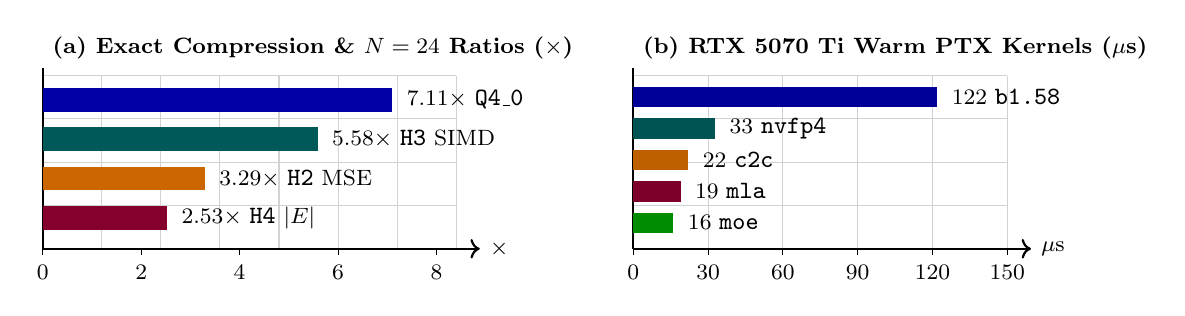
\begin{tikzpicture}[font=\footnotesize]
  % Panel A: N=24 & Exact Compression Factors
  \begin{scope}[xshift=0cm]
    \node[anchor=west] at (0, 2.55) {\textbf{(a) Exact Compression \& $N=24$ Ratios ($\times$)}};
    \draw[gray!35] (0,0) grid[xstep=0.75, ystep=0.55] (5.25,2.2);
    \draw[thick,->] (0,0) -- (5.55,0) node[right] {$\times$};
    \draw[thick] (0,0) -- (0,2.3);
    \fill[blue!65!black] (0,1.74) rectangle (4.44,2.04);
    \node[anchor=west] at (4.50,1.89) {$7.11\times$ \code{Q4\_0}};
    \fill[teal!70!black] (0,1.24) rectangle (3.49,1.54);
    \node[anchor=west] at (3.55,1.39) {$5.58\times$ \code{H3} SIMD};
    \fill[orange!80!black] (0,0.74) rectangle (2.06,1.04);
    \node[anchor=west] at (2.12,0.89) {$3.29\times$ \code{H2} MSE};
    \fill[purple!70!black] (0,0.24) rectangle (1.58,0.54);
    \node[anchor=west] at (1.64,0.39) {$2.53\times$ \code{H4} $|E|$};
    \foreach \x/\lbl in {0/0, 1.25/2, 2.50/4, 3.75/6, 5.00/8} {
      \draw (\x,0) -- (\x,-0.08) node[below] {\lbl};
    }
  \end{scope}

  % Panel B: Warm Blackwell PTX Kernel Latencies
  \begin{scope}[xshift=7.5cm]
    \node[anchor=west] at (0, 2.55) {\textbf{(b) RTX 5070 Ti Warm PTX Kernels ($\mu$s)}};
    \draw[gray!35] (0,0) grid[xstep=0.95, ystep=0.55] (4.75,2.2);
    \draw[thick,->] (0,0) -- (5.05,0) node[right] {$\mu$s};
    \draw[thick] (0,0) -- (0,2.3);
    \fill[blue!60!black] (0,1.80) rectangle (3.86,2.06);
    \node[anchor=west] at (3.92,1.93) {$122$ \code{b1.58}};
    \fill[teal!65!black] (0,1.40) rectangle (1.04,1.66);
    \node[anchor=west] at (1.10,1.53) {$33$ \code{nvfp4}};
    \fill[orange!75!black] (0,1.00) rectangle (0.70,1.26);
    \node[anchor=west] at (0.76,1.13) {$22$ \code{c2c}};
    \fill[purple!65!black] (0,0.60) rectangle (0.60,0.86);
    \node[anchor=west] at (0.66,0.73) {$19$ \code{mla}};
    \fill[green!55!black] (0,0.20) rectangle (0.51,0.46);
    \node[anchor=west] at (0.57,0.33) {$16$ \code{moe}};
    \foreach \x/\lbl in {0/0, 0.95/30, 1.90/60, 2.85/90, 3.80/120, 4.75/150} {
      \draw (\x,0) -- (\x,-0.08) node[below] {\lbl};
    }
  \end{scope}
\end{tikzpicture}
\caption{Verbatim \code{v1.0.0} performance receipts: (a)~exact \code{Q4\_0} compression ($64/9\times$) and pre-registered $N=24$ paired mean improvement ratios (\code{H2}--\code{H4}); (b)~warm dispatch latencies of all five verified Blackwell \code{sm\_12.0} PTX kernels (\code{probe}, pinned async paging $16.69\text{--}17.03\text{ GB/s}$).}
\label{fig:bench}
\end{figure}

\section{Six-Kernel Palomar Formal Verification in Pure Lean 4.35.0}
\label{sec:lean}

To preclude proof-statement tampering, vacuous hypotheses, and single-kernel
trust assumptions, \code{v1.0.0} refactors the formal proof suite into a modular
Lean~4.35.0 \code{module} architecture (\code{autoImplicit = false},
\code{relaxedAutoImplicit = false}, strict unused-variable and deprecation
linters, zero Mathlib) following the Palomar \code{Spec}/\code{Challenge}/\code{Solution}
contract:
\begin{itemize}
  \item \code{lean/BeastProofs/Spec.lean} \& \code{LiveReceiptData.lean}: pure
  shared definitions and hardware receipt constants (zero proofs, zero \code{sorry}).
  \item \code{lean/Challenge.lean}: imports \emph{only} \code{BeastProofs.Spec}
  and declares all $81$ target theorem types with \code{by sorry}, isolating the
  public specification from implementation tactics.
  \item \code{lean/Solution.lean} \& nine domain modules: sorry-free proofs of all
  $81$ declarations, including eight non-vacuity witnesses (\code{NV01}--\code{NV08})
  and eight adversarial false-variant refutations (\code{AT01}--\code{AT08}).
  \item \code{lean/comparator.json} \& \code{lean/VerifyAxioms.lean}: pins all
  $81$ \code{theorem\_names}, $10$ core \code{definition\_names}, and the $3$
  permitted standard axioms (\code{propext}, \code{Classical.choice},
  \code{Quot.sound}). Continuous integration executes \code{lake build},
  \code{leanchecker}, \code{leanchecker --paranoid}, \code{lake check --paranoid},
  \code{lake comparator --config comparator.json --paranoid} inside
  \code{bubblewrap} isolation, plus a live negative sorry-tamper comparator test
  and \code{scripts/test\_lean\_negative.py} ($3/3$ exploits mechanically rejected:
  \code{sorry}, custom \code{axiom}, and \code{native\_decide}).
\end{itemize}

Table~\ref{tab:lean} summarizes all $81$ audited declarations (verbatim
\code{\#print axioms} output is archived in \code{results/lean4-audit.txt} and
mirrored line-for-line in \code{README.md}).

\begin{table}[t]
\centering
\caption{Taxonomy and exact axiom footprint of all $81$ audited Pure Lean 4.35.0 declarations across all nine proof modules (\code{results/lean4-audit.txt}).}
\label{tab:lean}
\scriptsize
\begin{tabular}{@{} >{\raggedright\arraybackslash}p{3.0cm} >{\raggedright\arraybackslash}p{6.0cm} cc @{}}
\toprule
\textbf{Lean 4.35.0 Module} & \textbf{Verified Properties (\code{Spec.lean} Invariants)} & \textbf{Count} & \textbf{Axioms Used} \\
\midrule
\code{Quantization} & \code{B01}--\code{B05}, \code{B61}, \code{B64}: \code{b1.58} 243-state bijection, \code{NVFP4}/\code{u1}/\code{i2}, \code{Q4\_0} & 7 & $6$ zero-ax, $1$ \code{[p,Q]} \\
\code{CacheTelepathy} & \code{B06}--\code{B08}, \code{B18}, \code{B21}, \code{B30}: \code{Augment}, \code{SwaT}, spoof guard & 6 & $4$ zero-ax, $2$ \code{[p]} \\
\code{Ring0Security} & \code{B09}--\code{B10}, \code{B28}, \code{B38}, \code{B43}, \code{B62}: Ring-0 ACL, spend, Jobs, SSRF & 6 & $1$ zero-ax, $5$ std \\
\code{ColonyGovernance} & \code{B11}--\code{B16}, \code{B19}--\code{B20}, \code{B59}: NonHuman, ReZero, WSE, 300-matrix & 9 & $6$ zero-ax, $3$ \code{[p]} \\
\code{CryptoPhysics} & \code{B17}, \code{B22}, \code{B33}--\code{B35}, \code{B37}, \code{B40}--\code{B42}, \code{B45}--\code{B46}, \code{B50}, \code{B54}--\code{B56} & 15 & $7$ zero-ax, $8$ std \\
\code{SystemsRuntime} & \code{B23}--\code{B27}, \code{B31}--\code{B32}, \code{B44}, \code{B51}--\code{B53}: PTX, Multiboot1/2, GGUF, DSP & 11 & $9$ zero-ax, $2$ std \\
\code{LiveReceipt} & \code{B29}, \code{B36}, \code{B39}, \code{B47}--\code{B49}, \code{B57}--\code{B58}, \code{B60}, \code{B63}, \code{B65}: DLL/mutant/receipt & 11 & $11$ zero-ax \\
\code{NonVacuity} & \code{NV01}--\code{NV08}: concrete inhabited witnesses for key hypotheses & 8 & $7$ zero-ax, $1$ \code{[p]} \\
\code{AdversarialTests} & \code{AT01}--\code{AT08}: formal $\neg P$ refutations of broken/weakened variants & 8 & $4$ zero-ax, $4$ std \\
\midrule
\textbf{Total Audited} & \textbf{0 \code{sorry}, 0 custom axioms, 0 warnings, 6-kernel Palomar} & \textbf{81} & \textbf{55 zero-ax / 26 std} \\
\bottomrule
\end{tabular}
\end{table}

\subsection{Statement Fidelity and Standalone Model Transparency}
In keeping with strict proof-fidelity auditing (\code{docs/statement-fidelity.md}
and \code{ERRATA.md}), all $81$ Lean~4.35.0 declarations are \emph{standalone
formal models} in \code{Spec.lean}; no Lean module imports, extracts, or verifies
the shipped Rust, Zig, C11, or PTX source code. We explicitly partition all $81$
declarations into two mechanical tiers counted directly from \code{Challenge.lean}:
\begin{enumerate}
  \item \textbf{Quantified, Witness, and Refutation Declarations ($41$ declarations):}
  $25$ parameterized/quantified theorems over \code{Nat}, \code{Int}, \code{Fin 3},
  \code{BitVec 8}, \code{BitVec 64}, \code{List}, and the userland root-policy
  record \code{RootState} (\code{B02}, \code{B06}--\code{B07}, \code{B09}--\code{B13},
  \code{B17}--\code{B23}, \code{B25}, \code{B28}, \code{B35}, \code{B37}--\code{B38},
  \code{B45}, \code{B54}--\code{B56}, \code{B64}), plus $8$ non-vacuity witnesses
  (\code{NV01}--\code{NV08}) and $8$ formal negations (\code{AT01}--\code{AT08}).
  Note that \code{B09}--\code{B10} model a software root-policy guard (not CPU
  ring~0), and \code{B54}--\code{B55} prove \code{DualInt} multiplication and
  addition commutativity (not floating-point AD agreement).
  \item \textbf{Closed Ground and Committed Receipt-Constant Checks ($40$ declarations):}
  Spec size identities, checksums, bookkeeping sums, constant predicates
  (\code{B08}, \code{B43}, \code{B46}, \code{B62}), and committed receipt-constant
  consistency checks (\code{B60}, \code{B65}). In \code{v1.0.0}, the receipt
  exporter (\code{beast verify-all --export-lean}) writes \code{0} whenever a
  hardware backend is absent rather than substituting passing defaults; even so,
  \code{B60}/\code{B65} check consistency of committed constants in
  \code{LiveReceiptData.lean} and do \emph{not} prove inside the Lean kernel that
  external silicon executed.
\end{enumerate}

\section{Unsolved Problems Mega-Atlas (\texorpdfstring{\code{v2.8.0}}{v2.8.0}) Non-Retirement Cross-Check}
\label{sec:atlas}

To prevent scope inflation across adjacent open problems, we audited
\textsc{BEAST CIVILIZATION} \code{v1.0.0} verbatim against the
\code{unsolved-problems-mega-atlas} registry (\code{v2.8.0}, commit
\code{9e16554}, $1{,}900$ cataloged problems; \code{docs/MEGA\_ATLAS\_CROSSCHECK.md}).
\textbf{Headline verdict: $0 / 1{,}900$ overarching Mega-Atlas open problems are
solved or retired.} Table~\ref{tab:atlas} maps our scoped engineering and formal
constructions against the $10$ most closely adjacent catalog IDs.

\begin{table}[t]
\centering
\caption{Verbatim cross-check against $10$ adjacent Mega-Atlas \code{v2.8.0} (\code{9e16554}) open problems. All $10/10$ remain strictly \textbf{OPEN} ($0 / 1{,}900$ retired).}
\label{tab:atlas}
\scriptsize
\setlength{\tabcolsep}{4pt}
\begin{tabular}{@{} >{\raggedright\arraybackslash}p{1.45cm} >{\raggedright\arraybackslash}p{5.25cm} >{\raggedright\arraybackslash}p{4.3cm} >{\raggedright\arraybackslash}p{2.3cm} @{}}
\toprule
\textbf{Atlas ID} & \textbf{Verbatim Mega-Atlas \code{v2.8.0} Title} & \textbf{Scoped \code{beast-civilization} Construction} & \textbf{Parent Status} \\
\midrule
\code{LOG-033} & Lean Kernel Compilation vs.\ Human Statement Fidelity Verification Problem & Palomar \code{Challenge}/\code{Solution}, \code{NV01}--\code{NV08}, \code{AT01}--\code{AT08}, fidelity matrix & \textbf{OPEN} (0\% retired) \\
\code{AI-005} & Automated Formal Proof Fidelity Auditing (Lean 4 Kernel Verification vs.\ Human Statement Semantics) & 6-kernel \code{bubblewrap} CI + live sorry-tamper comparator rejection & \textbf{OPEN} (0\% retired) \\
\code{AI-051} & AI-Driven Self-Improvement Stability, Recursive Optimization Limits \& Intelligence Explosion Dynamics & Ring-0 ACL (\code{B09}), spend cap (\code{B10}), ReZero (\code{B12}), $\|W\|_2 \le 0.99$ (\code{B13}) & \textbf{OPEN} (0\% retired) \\
\code{CS-058} & Scalable End-to-End Formal Verification of Concurrent \& Cyber-Physical Software & Church--Rosser XOR (\code{B56}), Win32 Jobs (\code{G23}), QEMU ELF32 (\code{G17}) & \textbf{OPEN} (0\% retired) \\
\code{CS-059} & Automated Specification-Driven Program Synthesis \& Binary Equivalence Verification & Trinity Forge ELF32/A-Life synthesis + Prism-gated YARV breeder & \textbf{OPEN} (0\% retired) \\
\code{SYS-009} & Formal Cybernetic Theory of Multi-Scale Agency, Autopoiesis \& Self-Maintaining Systems & 3-colony $\times$ 6-caste OS, Planaria 50\% heal, 3$\times$ A-Life FFI~\cite{varela1974autopoiesis,levin2022tame} & \textbf{OPEN} (0\% retired) \\
\code{SYS-039} & Event-Triggered \& Neuromorphic Closed-Loop Control Achieving Sub-Millisecond Ultra-Low-Power Latency & $7.50\text{ ns}$ FFI, $16\text{--}122\,\mu\text{s}$ PTX kernels, \code{sLTC} liquid blocks & \textbf{OPEN} (0\% retired) \\
\code{HW-004} & Neuromorphic \& Analog In-Memory Hardware Matching Biological Synaptic Efficiency & \code{b1.58}/\code{NVFP4}/\code{Q4\_0} digital kernels + spintronic $p$-bit bridge & \textbf{OPEN} (0\% retired) \\
\code{QC-033} & Quantum Circuit Compilation, Routing \& Optimal T-Count / Clifford+T Synthesis Scaling & Classical C11 CHSH, QGT Chern/SSH/Kitaev, anyon \& Bloch verification & \textbf{OPEN} (0\% retired) \\
\code{CS-044} & Approximation Thresholds \& Coupled Dynamics for Equilibria Beyond PPAD & 6-variable cosine-schedule QUBO annealer (\code{H4}, \code{B19}) & \textbf{OPEN} (0\% retired) \\
\bottomrule
\end{tabular}
\end{table}

\section{Threats to Validity, Epistemic Boundaries, and Reproducibility}
\label{sec:boundaries}

\subsection{Threats to Validity and Honest Boundaries}
\begin{itemize}
  \item \textbf{Capability Matrix (\code{296 / 300} Verified, \code{4 / 300} \code{SPEC}):}
  \path{docs/matrices/300_agent_matrix.yaml} verifies $296$ entries live on
  hardware. Four entries remain honestly marked \code{SPEC}: \code{F036}
  (\code{tsotchke/tensorcore} targets Apple Silicon Metal/Accelerate rather than
  Win64 x86-64), and \code{F038}, \code{F068}, \code{F069} (external multi-gigabyte
  HuggingFace, Whisper, Kokoro, and TFLite checkpoints are intentionally omitted;
  zero-weight deterministic DSP ASR/TTS and noisy 2D Sobel/\code{b1.58} OCR run
  locally instead).
  \item \textbf{External Validity of Small-Scale Benchmarks:} Our 4-layer
  \code{GQA}$\to$\code{Chimera} C2C bridge ($142{,}496\text{ B}$), 6-variable QUBO
  annealer, and 10-block Chimera breeder demonstrate exact end-to-end mechanics and
  statistically significant paired gains at local workstation scale; scaling to
  frontier multi-billion-parameter LLMs requires distributed VRAM and remains
  future work.
  \item \textbf{Single-Host GPU Timing and CRuby YJIT:} Blackwell \code{sm\_12.0}
  measurements reflect one RTX 5070 Ti host and exhibit cold-JIT vs.\ warm-dispatch
  variance; GitHub Actions Ubuntu/Windows/macOS runners execute the full CPU,
  Rust, Zig, C11 ASan/UBSan, CRuby, Python oracle, and 6-kernel Lean pipelines
  without GPU silicon. Local RubyInstaller~3.4.9 ships with \code{+PRISM} and
  \code{YJIT=false}.
  \item \textbf{Zero Anthropomorphism:} Multi-colony and Planaria terminology
  denotes deterministic software scheduling, erasure coding, and Merkle verification
  with zero claims of sentience, consciousness, or physical wet-lab proof.
\end{itemize}

\subsection{Reproducibility and Artifact Preservation}
All builds, statistics, oracle checks, negative tests, and this PDF reproduce from
a clean clone via \code{just reproduce} (or \code{.\textbackslash build.ps1} on
Windows). Cryptographic integrity is anchored by \path{CHECKSUMS.sha256},
\path{results/MANIFEST.sha256}, \path{data/MANIFEST.sha256}, an RFC~3161 DigiCert
timestamp token (\path{data/timestamps/CHECKSUMS.sha256.tsr}), GitHub SLSA v4
build-provenance attestations, and Software Heritage archival.

\subsection{CRediT Author Contributions, Ethics, and AI-Assistance Disclosure}
\textbf{Author Contributions (CRediT):} Alexander Stephen Donahue (ORCID
\code{0009-0006-8168-9648}) conceived the architecture, directed all software
engineering, formal verification, statistical evaluation, and manuscript drafting,
and takes sole responsibility for all claims and errors.
\textbf{Conflicts of Interest \& Funding:} None declared; independent unfunded
research.
\textbf{Data \& Code Availability:} All source code, Lean~4 proofs, scripts, raw
$N=24$ outputs, and machine-readable citation audit
(\code{results/citation-audit.json}) are publicly available at
\url{https://github.com/0thernes/beast-civilization} (code/Lean: Apache-2.0;
manuscript/docs: CC BY 4.0).
\textbf{AI-Assistance Disclosure:} AI coding and proof assistants were used during
implementation, Lean proof drafting, adversarial code auditing, and LaTeX
typesetting under continuous human direction. Correctness of all $81$ formal
declarations is certified independently by six deterministic Lean~4.35.0 proof
kernels (zero \code{sorry}, strictly standard axioms), and correctness of all
empirical and statistical receipts is independently reproducible from raw source
code rather than by authoring provenance.

\bibliographystyle{plainurl}
\bibliography{refs}

\end{document}
